
\documentclass [PhD] {uclathes}

% \input {mymacros}                         % personal LaTeX macros

%%%%%%%%%%%%%%%%%%%%%%%%%%%%%%%%%%%%%%%%%%%%%%%%%%%%%%%%%%%%%%%%%%%%%%
%
% Usually things live in separate flies.
%
% \input {prelim}                           % preliminary page info

%%%%%%%%%%%%%%%%%%%%%%%%%%%%%%%%%%%%%%%%%%%%%%%%%%%%%%%%%%%%%%%%%%%%%%%%
%                                                                      %
%                          PRELIMINARY PAGES                           %
%                                                                      %
%%%%%%%%%%%%%%%%%%%%%%%%%%%%%%%%%%%%%%%%%%%%%%%%%%%%%%%%%%%%%%%%%%%%%%%%

\title          {Improving the Throughput \\
	of Connectionless Datagram Protocols \\
	over Networks with Limited Bandwidth}
\author         {Richard Bert Wales}
\department     {Computer Science}
% Note:  degreeyear should be optional, but as of  5-Feb-96
% it seems required or you get a year of ``2''.   -johnh
\degreeyear     {1993}

%%%%%%%%%%%%%%%%%%%%%%%%%%%%%%%%%%%%%%%%%%%%%%%%%%%%%%%%%%%%%%%%%%%%%%%%

\chair          {Jack W.\ Carlyle}
\member         {Mario Gerla}
\member         {David G.\ Cantor}
\member         {Richard L.\ Baker}
\member         {Robert M.\ Stevenson}

%%%%%%%%%%%%%%%%%%%%%%%%%%%%%%%%%%%%%%%%%%%%%%%%%%%%%%%%%%%%%%%%%%%%%%%%

\dedication     {\textsl{To my mother \ldots \\
		who---among so many other things--- \\
		saw to it that I learned to touch-type \\
		while I was still in elementary school}}

%%%%%%%%%%%%%%%%%%%%%%%%%%%%%%%%%%%%%%%%%%%%%%%%%%%%%%%%%%%%%%%%%%%%%%%%

\acknowledgments {(Acknowledgments omitted for brevity.)}

%%%%%%%%%%%%%%%%%%%%%%%%%%%%%%%%%%%%%%%%%%%%%%%%%%%%%%%%%%%%%%%%%%%%%%%%

\publication    {\textsl{MADHOUS Reference Manual.}
	Stanford University, Dean of Student Affairs
	(Residential Education Division), 1978.
	Technical documentation for the MADHOUS
	software system used to assign students to
	on-campus housing.}

%%%%%%%%%%%%%%%%%%%%%%%%%%%%%%%%%%%%%%%%%%%%%%%%%%%%%%%%%%%%%%%%%%%%%%%%

\abstract       {(Abstract omitted for brevity)}

%%%%%%%%%%%%%%%%%%%%%%%%%%%%%%%%%%%%%%%%%%%%%%%%%%%%%%%%%%%%%%%%%%%%%%%%



\begin {document}
\makeintropages

%%%%%%%%%%%%%%%%%%%%%%%%%%%%%%%%%%%%%%%%%%%%%%%%%%%%%%%%%%%%%%%%%%%%%%
%
% Ordinarily each chapter (at least) is in a separate file.
%
%
% introduction.tex
% Copyright (C) 2021 by Krish Kabra, <krish@kabra.com>.
%

\chapter{Introduction} \label{chap:intro}

\begin{figure}
    \centering
    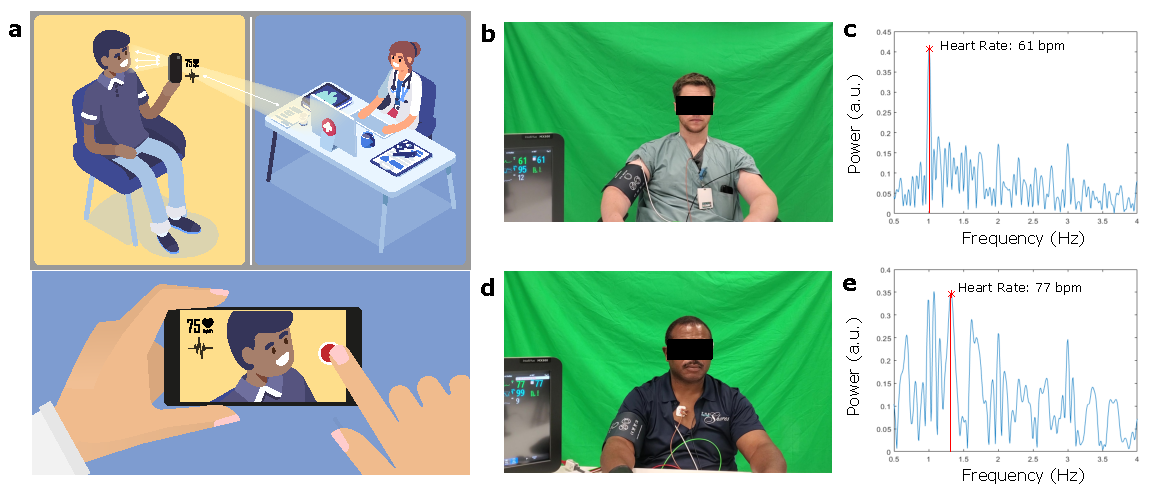
\includegraphics[width=\linewidth]{include/intro-fig.pdf}
    \caption{\textbf{Translating contactless camera-based HR sensing for telemedicine will require mitigating biased performance against dark skin tones.} (a) Cartoon illustration depicting the telemedicine application for the proposed contactless camera-based HR estimation. Telemedicine video-conferencing applications can be integrated with a software toolkit to display patient pulsatile signal and HR. (b) Frame of light skin tone subject from video. (c) Power spectrum of estimated pulsatile signal from light skin tone subject. Distinct peak at correct HR is shown in red. (d) Frame of dark skin tone subject from video. (e) Power spectrum of estimated pulsatile signal from dark skin tone subject. Frequency peak corresponding to correct HR is surrounded by noisy peaks. Videos used originate from the VITAL dataset. The CHROM algorithm with facial aggregation is employed to estimate the pulsatile signal. Credits: Illustration by Shelly Recchio.}
    \label{fig:teaser}
\end{figure}

Heart rate (HR) is an important clinical vital sign used in the evaluation of cardiorespiratory and hemodynamic stability. Conventional HR assessment is performed in-person at a clinic or hospital using specialized monitoring equipment. However, in recent years, healthcare delivery has progressed towards a remote model that uses telemedicine and mobile health (mHealth) technologies for patient evaluations. This transition has been accelerated by the COVID-19 pandemic \cite{annis_rapid_2020,ford_leveraging_2020,connolly_rapid_2020} in order to protect patients and healthcare workers from infectious exposure in a pandemic setting. The assessment of HR in patients with suspected COVID-19 is particularly important as COVID-19 has been associated with pre-existing cardiovascular disease \cite{nishiga_covid-19_2020}. Given the clinical relevance of HR in triage decisions, diagnosis, prognosis, and as a criterion for transfer to higher-level medical care, there is a pressing need to develop HR sensing solutions that can facilitate the rapidly growing domain of telemedicine-based care and remote patient monitoring.

Presently, HR sensing solutions for telemedicine and remote patient monitoring have relied on the adoption of wearable sensors to make plethysmographic or electrocardiographic measurements \cite{dinh-le_wearable_2019,lukas_emerging_2020}. Although such wearable technologies have seen major advances in the past decade \cite{kumar_mobile_2013, steinhubl_emerging_2015}, they still require large expenditure on production and distribution of hardware. This expense can create a barrier to adoption of mHealth technologies that disproportionately affects rural and socioeconomically burdened communities \cite{sawyer_wearable_2020}. 

In contrast to wearable sensors, recent methods have proposed using camera-based hardware present on modern-day smartphones in combination with signal processing and computer vision algorithms to estimate key vital signs, including HR \cite{li_current_2019}. Given the high penetration of mobile phone technology globally \cite{pew_demographics_2019}, such a solution would potentially have zero marginal cost, thereby offering clinicians a highly accessible and inexpensive method of assessing vital signs remotely. 

Camera-based HR sensing methods can be categorized into two distinct methodologies: contact-based and contactless. Contact-based methods, where the finger is typically placed on top the camera module, have already seen widespread applications in major smartphones \cite{proesmans_mobile_2019,li_current_2019}. Such methods show good performance, however, their utility for telemedicine video-conferencing visits is potentially limited as the camera module is covered during measurement. This prevents continuous monitoring of patient HR, visual well-being, and collection of other vitals such as respiratory rate and spatial blood perfusion maps. Contactless methods circumvent this limitation by remotely extracting a blood volume pulse (BVP) signal and corresponding HR estimate traditionally from facial videos \cite{rouast_remote_2018}. The consequence of capturing a larger field-of-view is a much weaker signal, and therefore worse performance. 

Remote photoplethysmography (R-PPG) is by far the most prominent technique used in literature for contactless camera-based HR sensing. R-PPG operates by looking for subtle color variations visible on the surface of human skin, caused by sub-dermal light absorption fluctuations from changes in blood volume and content. Early work conducted by Verkruysse \textit{et al.} \cite{verkruysse_remote_2008} showed that plethysmographic signals could be measured using ambient light and a consumer-grade digital camera. In order to accurately isolate and extract the correct BVP signal corresponding to the HR, several R-PPG algorithms have been proposed, including blind source separation (BSS)~\cite{poh_noncontact_2010,tsouri_constrained_2012,lewandowska_measuring_2011}, model-based~\cite{haan_robust_2013,wang_algorithmic_2017,song_new_2020,de_haan_improved_2014}, unsupervised data-driven~\cite{wang_novel_2016,tulyakov_self-adaptive_2016}, and supervised deep learning~\cite{chen_deepphys_2018,niu_rhythmnet_2020,yu_remote_2019,yu_remote_2019-1,nowara_benefit_2020,spetlik_visual_2018} methods. Unfortunately, the performance of existing R-PPG algorithms fluctuates with changes in illumination condition \cite{li_remote_2014}, subject motion \cite{mocco_motion_2016,de_haan_improved_2014,wang_exploiting_2015}, and skin tone \cite{nowara_meta-analysis_2020}. Moreover, assessment of these algorithms has typically been done on computer vision datasets that are not focused on telemedicine applications. Consequently, these datasets do not represent characteristics that are important for clinical translation such as a large population with diverse skin tone and gender representation and video data collection on end-user devices such as smartphones. 

The focus of this thesis is on developing a contactless camera-based HR sensing method for smartphone deployment that can successfully translate to telemedicine application. In particular, this thesis specifically addresses the bias for skin tone present in R-PPG algorithms. We provide a theoretical framework to understand the unique physics that underlies the inconsistency in R-PPG measurement across skin tones. From this, we establish that the bias is due to imaging noise, and appropriately propose R-PPG denoising methods to alleviate performance losses, including a novel algorithm that achieves overall state-of-the-art performance and large performance gains for dark skin tones. To assess the performance of the proposed method, we collect the first remote vital signs detection dataset focused on telemedicine applications that is demographically diverse. 

\section{Contributions}

In context of prior R-PPG related works, this thesis demonstrates the following technical contributions:

\begin{enumerate}
    \item A light-transport theory for R-PPG application that provides novel mathematical insights of R-PPG performance and biases with respect to skin tone.
    \item The first clinical telemedicine-focused remote vital signs dataset, named VITAL, that contains a diverse population of subjects under a variety of recording conditions. 
    \item A novel R-PPG algorithm that achieves overall state-of-the-art performance and large performance gains for dark skin tones on the VITAL dataset.
\end{enumerate}

% \section{Organization}


                         


\bibliographystyle{IEEEtran}
\bibliography{references}    % bibliography references

\end {document}